\section{Hour Estimation}

	This section describes what hour estimation is, how to perform it and how we
	included it in our project. The actual estimated hours are not done in this section, 
	but is documented in each sprint section.

	{\bf What is hour estimation?} Hour estimation is performed as a part of a project in order to ensure that 
	one have the resources necessary to complete a project in time. Hour estimation can be done in many different 
	ways, but often depends on the methodology	used in the project. In a waterfall project, it is common to do all 
	the estimation in the start of a project. When a project uses agile methods like scrum, it is common to do 
	the estimation partin each sprint. \cite{estimation}

	{\bf Why perform hour estimation?} In software projects, the projects normally starts with
	a planning phase and an hour estimation. There are several reasons as to why this estimation is done:
		\begin{itemize}
			\item Calculate the cost for delivering a project.
			\item Calculation resources for a project (e.g how many people do the team 
			need for this project?).
			\item How many features can the team implement during a phase/sprint?
			\item Are the project in time (the estimated hours in the backlog)?
			\item How big is this project in terms of hours?
		\end{itemize}
	There are many good reasons for doing an estimation, but the reasons are often dependent
	on the methodology used and the purpose of the project. 

	If no estimation has been performed in a project, there are many risk factors that can appear:
	\begin{itemize}
		\item If a company win a project and promises the customer to deliver at a 
		specified date without estimating hours for the project, there is a big risk 
		that the project will fail.
		\item If a project has not estimated the hours, there is a possibility that 
		there is not allocated enough resources for the project, and the project could 
		be risking not to be delivered at the planned date.  
	\end{itemize}

	{\bf How we performed hour estimation} This project have like many other projects a deadline
	as well as a specified number of resources. In many projects it is normal to set the wanted 
	delivery and then estimate the number of resources needed to deliver the project.
	In this project we started with a number of resources (4 students) and then planned the 
	delivery based on the workload of the course (ca 24 hours/persons/week). The actual 
	hour estimation is done in the start of every sprint. The reason for doing this is because of 
	the chosen methodology scrum.

	\begin{figure}[H]
		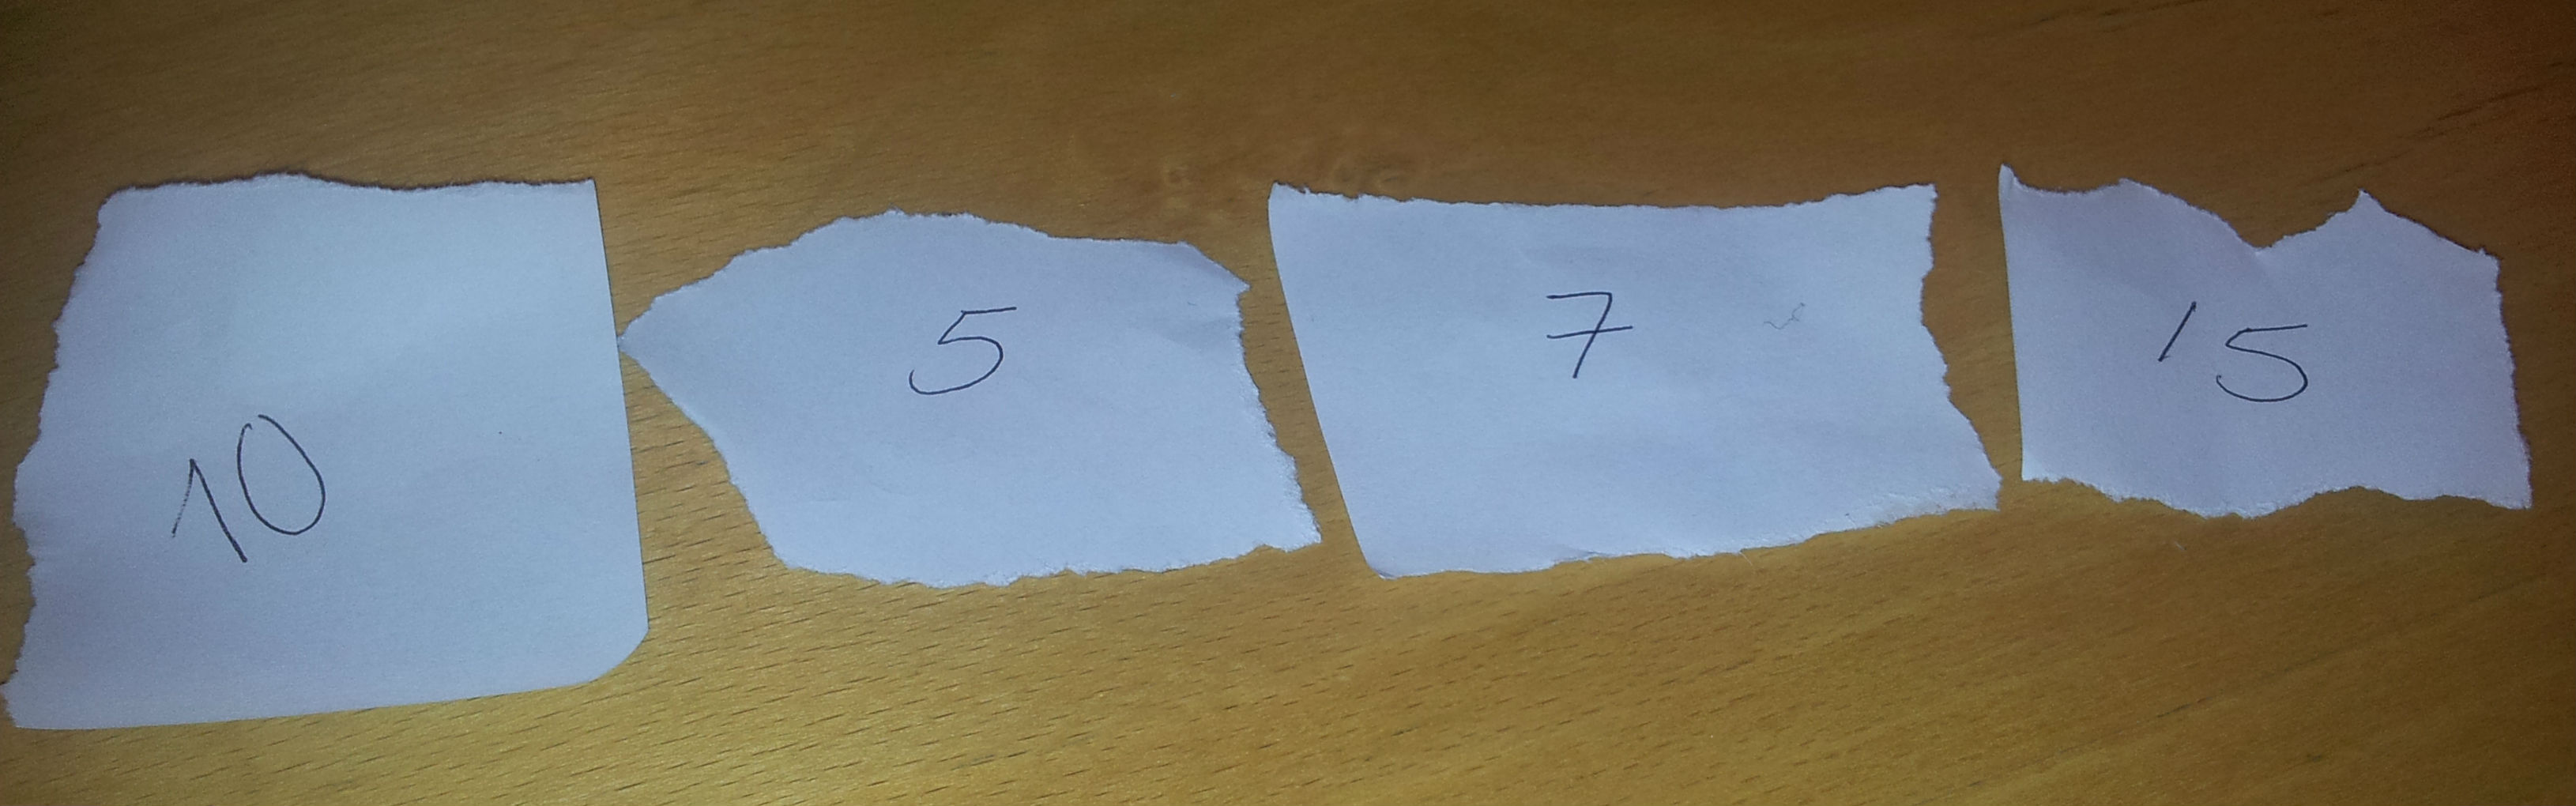
\includegraphics[width=1.0\textwidth]{pictures/estimation.jpg}
		\caption{Hour estimation from sprint 2}
	\end{figure}

	In the start of every sprint, the group performed hour estimation for the sprint.
	Before the hour estimation, the sprint backlog was planned. For every functional requirement
	in the sprint backlog, every person in the scrum team wrote down a guessed hour estimate
	for the requirement. After showing all the estimates, we chose the average of
	the estimates. The reason for doing it this way was because the group 
	was quite unexperienced with hour estimation. When doing it this way, some team 
	members will overestimate and some will underestimate and the result will often be an estimate 
	that is close to the actual effort. 
